\chapter{Sequence models}

Next, we will implement models which take the ordering of tokens into
account. This includes \acp{CNN} and \acp{RNN}. In \ac{NLP}, \acp{CNN} can be
considered as a ``\ngram extractor'', which looks at a window of tokens.
However, unlike the count vector approach used above, the CNN extracts
``soft'' \ngrams, utilizing the ability of word embeddings to share
statistical strength between words, and outputting a real-valued number
instead of a boolean yes/no value or an integer count.

\acp{RNN} are theoretically able to detect long range patterns, which seems
like it would be useful for the tasks at hand. For instance, the ability to
connect different sections of a text and refer back to things that have been
mentioned before can be considered a part of language proficiency.


\section{Experimental setup}

Certain aspects of setup are shared between experiments using \ac{CNN} and
\ac{RNN} models.

\subsection{Input length}

The models in this chapter take as input a document of a predetermined
length. We therefore needed to set a fixed number of tokens such that shorter
documents were padded to this length, and longer documents truncated. In
order to decide this, we examined the distribution of document lengths in the
training set. All subsequent values are rounded to the nearest integer.
First, we found the 95th percentile of document lengths, which turned out to
be 701 tokens. Then, we computed the value $Q_2 + 1.5 \cdot (Q_3 - Q_1)$, or
the median plus 1.5 times the interquartile range, which gives 693 tokens.
Finally, we computed the mean value plus two standard deviations, giving 707
tokens. These values are all close to each other, and we decided to settle on
700 tokens since it is a round number close to all values we examined.

As a consequence of the unequal distributions of length between the two test
levels, the documents that are truncated are mainly from the AL test. This
could be problematic if the 


\subsection{Pre-trained embeddings}

We experimented with randomly initialized word embedding vectors trained from
scratch, as well as initializing the vectors with pre-trained embeddings.In
this case, the embeddings came from different models trained on a large
Norwegian corpus, the combination of Norsk aviskorpus and NoWaC (Norwegian
Web As Corpus). The FastText algorithm lets us use these models to compute
vectors for words that do not have entries in the model, by instead basing
the vector on the word's character \ngrams.

These vector models are very large, containing vectors for more than
2,500,000 words. Our training data only contains 18,305 unique tokens, and
loading the full pre-trained model takes a long time and uses huge amounts of
memory for word vectors we will never use. For that reason, we created models
of smaller size by loading the full models once and iterating through all of
the word forms in our corpus, storing the resulting vectors in a new vector
model containing only 18,305 words. In this way, we are also able to benefit
from the FastText models' ability to compute vectors for unknown words, since
the \ngram algorithm is being used when computing the reduced models.
However, the fine-tuning of vectors happens no different from if we had used
embeddings from simpler models such as Word2vec, since the FastText network
is not incorporated into our models.

When using pre-trained embeddings, we ran some experiments keeping the
embeddings static, and some where we further fine-tuned the embeddings using
training signals from the task.

\subsection{Multi-channel input}

For some of our experiments we use both word tokens and their POS tags as
input at the same time. To do this we include two separate embedding matrices
in our network, one for words and one for POS tags. These embedding matrices
do not need to have the same dimensionalities, and because the number of
different POS tags is very low compared to the number of different words, we
use smaller vectors for POS tags.

To create the input to the core part of our network, we concatenate the word
and POS embeddings into a single vector. For instance, if we use word
embeddings of size 50 and POS embeddings of size 10, the next layer will
receive vectors of size 60.


\section{Convolutional neural networks}

We create a model with convolutional architecture based on the model
described in \textcite{kim2014convolutional}. Documents are represented as
sequences of token IDs, and fed into an embedding lookup layer. A separate
token ID is used for padding if the document is shorter than 700 tokens.
Another unique token ID is used for unknown tokens, i.e. tokens that either
are not present in training data, or are not among the $n$ most frequent
tokens, if we select a frequency cutoff.

The central part of the architecture is a set of convolutional filter banks
that are applied to sequences of embeddings. We may use several different
window sizes for the filters. The default architecture from
\textcite{kim2014convolutional} uses 300 convolutional filters: 100 each of
window size 3, 4 and 5. After applying the convolutions, the output is max
pooled along the time axis. This selects the highest output each filter
computed across all windows in the document. In practice, three pooling
operations are included in the computational graph, one for each filter bank.
This is a technical consideration, necessary because of the different window
sizes. The pooled vectors for each of the filter banks are concatenated into
a single vector. This vector has as many elements as there are filters in all
the filter banks combined.

The vector post-pooling is a vector representation of the entire document,
and is fed to a final softmax layer to produce a classification output.
During training, we apply dropout to this final weight layer as a
regularization method.


\subsection{Results}

The \ac{CNN} classifier that used both tokens and POS tags as input performed
better than the one which only used tokens as input, as seen in table
\ref{tab:cnn-results}. However, on the collapsed label set, the model which
only used tokens had a higher accuracy. Filters of size 3, 4, and 5 were
used. The last dense layer uses dropout with $p=0.5$ and a constraint on
maximum $L_2$ norm of 3.

\begin{table}
  \centering
  \begin{tabular}{lrrrr}
    \toprule
            & \multicolumn{2}{c}{All labels}       & \multicolumn{2}{c}{Collapsed labels} \\
    \cmidrule(lr){2-3}
    \cmidrule(lr){4-5}
    Model     & Macro \FI        & Micro \FI        & Macro \FI        & Micro \FI \\
    \midrule
    %           cnn-26092298_01                       cnn-26092298_02
    Words     &         $0.226$  &         $0.415$  &         $0.397$  &         $0.748$  \\
    %           cnn-26092298_03                       cnn-26092298_04
    Words+PTD &         $0.238$  &         $0.390$  &         $0.375$  &         $0.707$  \\
    %           cnn-26092298_05                       cnn-26092298_06
    Words+PTS &         $0.226$  &         $0.390$  &         $0.392$  &         $0.740$  \\
    %           cnn-26092298_07                       cnn-26092298_08
    +POS      &         $0.228$  &         $0.390$  &         $0.402$  &         $0.756$  \\
    %           cnn-26092298_09                       cnn-26092298_10
    +POS+PTD  &         $0.229$  &         $0.415$  &         $0.388$  &         $0.732$  \\
    %           cnn-26092298_11                       cnn-26092298_12
    +POS+PTS  &         $0.201$  &         $0.382$  &         $0.426$  &         $0.740$  \\
    %           cnn-26093545_13                       cnn-26093545_14
    Mix       &         $00000$  &         $00000$  &         $00000$  &         $00000$  \\
    %           cnn-26093545_15                       cnn-26093545_16
    Mix 234   &         $00000$  &         $00000$  &         $00000$  &         $00000$  \\
    \bottomrule
  \end{tabular}
  \caption{\FI scores of CNN classifiers on AES. +POS: Multi-channel input with
           both words and POS tags. +PTD: Pre-trained word embeddings, further
           fine-tuning. +PTS: Pre-trained word embeddings kept static. 234:
           filter widths 2, 3 and 4.}
  \label{tab:cnn-results}
\end{table}


\subsection{Training behaviour}

\begin{figure}
  % cnn-26092298_03
  \centering
  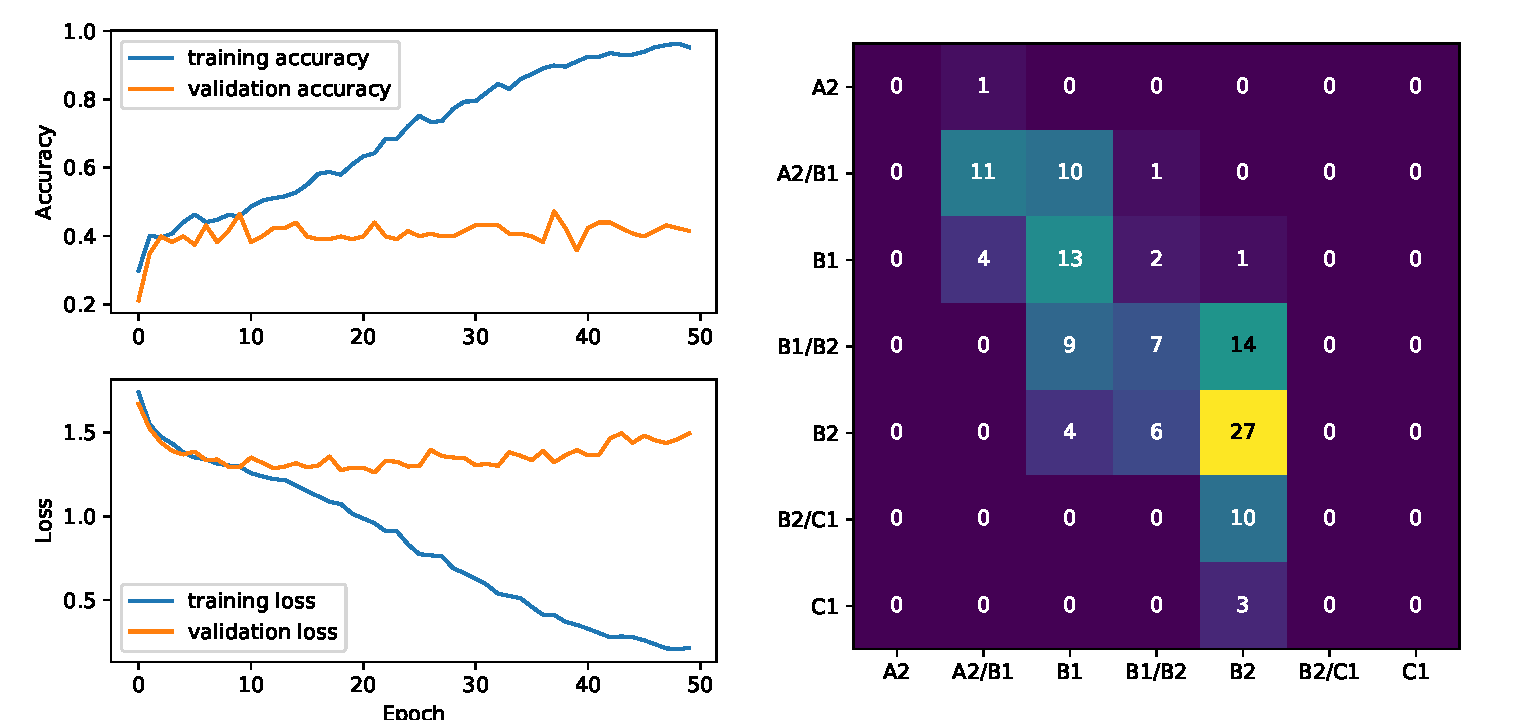
\includegraphics[width=\textwidth]{cnn-training}
  \caption{Training and validation loss and accuracy over 50 epochs of training.
           Also, confusion matrices with counts and normalized by class.}
  \label{fig:cnn-training}
\end{figure}

Figure \ref{fig:cnn-training} shows that the best performing model overfits
the training data. While the validation metrics plateau after approximately
10 epochs, after which we see only small, seemingly random fluctuations.
The training metrics keep improving, suggesting that the model is memorizing
the data rather than discovering general features. After roughly 25 epochs,
the training accuracy reaches almost 100\% and stays there.


\section{Recurrent neural networks}

A \ac{LSTM} \ac{RNN} was implemented based on the architecture described by
\textcite{taghipour16}. Several changes to their architecture were made in
order to accomodate our data. For instance, \citeauthor{taghipour16} modelled
the task as a regression problem, their output layer consisting of a single
node with a value constrained to (0, 1) by the sigmoid function. This layer
was replaced with a softmax layer similar to the \acp{MLP} in section
\ref{subsec:mlp}.

We then chose a loss function to be compatible with a multi-class softmax
output. Like above, we used categorical cross-entropy (equation
\ref{eq:crossentropy}). A different evaluation metric was also needed because
we are treating the task as multi-class prediction. We are reporting macro
and micro \FI as before. We do not use the \ac{QWK} metric used by
\citeauthor{taghipour16}. \todo{why not QWK}

The formulation of the \ac{AES} task as a regression problem by
\citeauthor{taghipour16} was partly a constraint stemming from the Kaggle
competition that supplied the data and problem formulation, and partly
motivated by the nature of the data. The ASAP data consists of essays from
eight different prompts, and the scoring methods differs across prompts.
Since the scores are numeric values over different ranges, modelling the task
as a regression problem made it sufficient to normalize the numeric scores to
a common interval before training.

Generally for \ac{AES}, modelling the task as multi-class prediction is
common, and is used in \autocite{vajjala18universalCEFR}. In
\autocite{vajjala17}, two different datasets with different properties were
used, and the author utilized both multi-class prediction and regression at
different points.

The embedding layer in \textcite{taghipour16} was initialized with
pre-trained embeddings of size 50. Our embedding layer was initialized to
random vectors and trained as part of the network.

Unlike our corpus, ASK, the dataset used by \citeauthor{taghipour16}
contained essays that were not necessarily written in a second language. Our
data is not split into different parts based on the prompt. There are two
different test levels in ASK, but these are not distinguished in training.

Note that the activation function for the gates in gated RNNs in Keras by
default is the \emph{Hard sigmoid} activation function (ref. eq.
\ref{eq:hardsigmoid}), chosen because it is computationally more efficient
than the sigmoid function.

We also experimented with a different type of gated \ac{RNN} cell, the
\ac{GRU}. This variant of \ac{RNN} is slightly simpler than the \ac{LSTM},
featuring only two gates. However, it is still designed to be able to
propagate the error gradient over a larger number of timesteps, like
\ac{LSTM}. In this way the architecture is supposed to mitigate the problem
of vanishing or exploding gradients. The equations defining \ac{LSTM}
\ac{GRU} cells are listed in chapter \ref{ch:background}, equations
\ref{eq:lstm} and \ref{eq:gru}.


\subsection{Variants}

We attempt two different methods of combining the sequence of hidden states
from the \ac{RNN} into a feature vector. The simplest approach is \emph{mean
over time}, where we use the elementwise average of elements in hidden states
across the time dimension as our feature vector. The mean over time layer is
used in two of the experiments. Once with a \ac{RNN} processing the essay
from top to bottom, and once on top of a bidirectional RNN.

The bidirectional model (BiRNN) is constructed by running two \acp{RNN} over
the same input, but in the opposite order. The output from the BiRNN layer is
a sequence of vectors where, for each timestep $j$, the vector is the
concatenation of two vectors $[s_f;s_b]$ where $s_f$ at timestep $j$ is the
output from the forwards \ac{RNN} after processing the inputs $(x_1, x_2,
\ldots, x_j)$ and $s_b$ the output from the backwards \ac{RNN} after
processing the inputs $(x_m, x_{m-1}, \ldots, x_j)$, where $m$ is the total
number of timesteps. The BiRNN should therefore be able to extract context on
both sides of a input timestep.

\todo{Mean of the final state}
\todo{Add POS inputs to RNN}

The attention model uses an attention layer, which differs from the mean over
time layer in that timesteps are weighted by an attention mechanism: a
single-layer neural network computes a value between -1 and 1 for each
timestep. These values are normalized by a softmax layer and then used to
compute the weighted average. Since each timestep contributes to the final
representation in differing amounts, the mechanism should be able in theory
to focus on crucial information by choosing weights such as to disregard
uninformative timesteps, improving performance. The attention mechanism is
trained along with the rest of the network.

All the models a hidden state vector of size 300 in the \ac{RNN}. The
vocabulary was limited to the 4,000 most common words, the same vocabulary
size as is used in \textcite{taghipour16}.


\subsection{Results}

Results for four different models are shown in table \ref{tab:rnn-results}.
Except where noted, hyperparameters match \textcite{taghipour16}. The
\emph{Attention} models do not use masking, while \emph{Mean/Time} and
\emph{BiLSTM} do. \todo{Always use pre-trained embeddings when repeating the
experiments?}

\begin{table}
  \centering
  \begin{tabular}{lrrrr}
    \toprule
            & \multicolumn{2}{c}{All labels} & \multicolumn{2}{c}{Collapsed labels} \\
    \cmidrule(lr){2-3}
    \cmidrule(lr){4-5}
    Model     & Macro \FI      & Micro \FI      & Macro \FI      & Micro \FI \\
    \midrule
              \multicolumn{5}{c}{50 dimensional, randomly initialized embeddings} \\
    \midrule
    % 50 dim, random init
    %           taghipour_ng-2019-01-15_20-50-06      taghipour_ng-2019-01-15_20-46-42
    Mean/Time &         $0.280$  &         $0.382$  &         $0.461$  &         $0.699$  \\
    %           taghipour_ng-2019-01-22_12-58-00      taghipour_ng-2019-01-22_13-01-44
    BiLSTM    &         $0.286$  &         $0.398$  &         $0.485$  &         $0.683$  \\
    %           rnn-25832764                          rnn-25832765
    Attention &         $0.244$  & $\mathbf{0.423}$ &         $0.559$  &         $0.780$  \\
    \midrule
    % 50 dim, pretrained, fine tune
              \multicolumn{5}{c}{50 dimensional, pre-trained embeddings, w/ fine tuning} \\
    \midrule
    %           rnn-25832746                          rnn-25832747
    Mean/Time &         $0.285$  &         $0.415$  &         $0.466$  &         $0.659$  \\
    %           rnn-25832748                          rnn-25832749
    BiLSTM    &         $0.257$  &         $0.374$  &         $0.447$  &         $0.691$  \\
    %           taghipour_ng-2019-01-24_19-16-41      taghipour_ng-2019-01-24_21-23-34
    Attention &         $0.303$  &         $0.423$  &         $0.558$  & $\mathbf{0.805}$ \\
    \midrule
    % 100 dim, pretrained, fine tune
              \multicolumn{5}{c}{100 dimensional, pre-trained embeddings, w/ fine tuning} \\
    \midrule
    %           rnn-25832716                          rnn-25832717
    Mean/Time &         $0.271$  &         $0.390$  &         $0.496$  &         $0.724$  \\
    %           rnn-25831870                          rnn-25831871
    BiLSTM    &         $0.301$  &         $0.350$  &         $0.456$  &         $0.683$  \\
    %           rnn-25832718                          rnn-25832719
    Attention &         $0.288$  &         $0.398$  &         $0.538$  &         $0.797$  \\
    \midrule
    % GRU cells, attention
              \multicolumn{5}{c}{GRU cells with attention} \\
    \midrule
    %           rnn-25858207                          rnn-25858208
    Rnd. init &         $0.299$  &         $0.431$  &         $0.533$  &         $0.764$  \\
    %           rnn-25858209                          rnn-25858211
    Pre train & $\mathbf{0.354}$ &         $0.390$  &         $0.493$  &         $0.724$  \\
    \midrule
    % LSTM cells, attention, frozen embeddings
              \multicolumn{5}{c}{LSTM + Attention with pre-trained, static embeddings} \\
    \midrule
    %           rnn-25858349                          rnn-25858350
    50 dim    &         $0.261$  & $\mathbf{0.488}$ &         $0.511$  &         $0.772$  \\
    %           rnn-25858483                          rnn-25858494
    100 dim   &         $0.271$  &         $0.472$  &         $0.491$  &         $0.707$  \\
    \midrule
    % LSTM cells, POS as additional input, attention
              \multicolumn{5}{c}{POS included with input} \\
    \midrule
    %           rnn-25985449                          rnn-25985450
    Rnd. init &         $0.261$  &         $0.366$  &         $0.552$  &         $0.780$  \\
    %           rnn-25985451                          rnn-25985452
    Pre train &         $0.277$  &         $0.407$  & $\mathbf{0.624}$ &         $0.756$  \\
    \bottomrule
  \end{tabular}
  \caption{\FI scores of RNN classifiers on AES}
  \label{tab:rnn-results}
\end{table}
\todo{300-dim embs: ran out of memory}

We find that the best performing models all use the attention mechanism.
Keep in mind that the stopping criterion is the macro \FI score, and thus
the micro \FI score is to be considered a side effect of the macro \FI.

\subsection{Training behaviour}

\begin{figure}
  % rnn-25858209
  \centering
  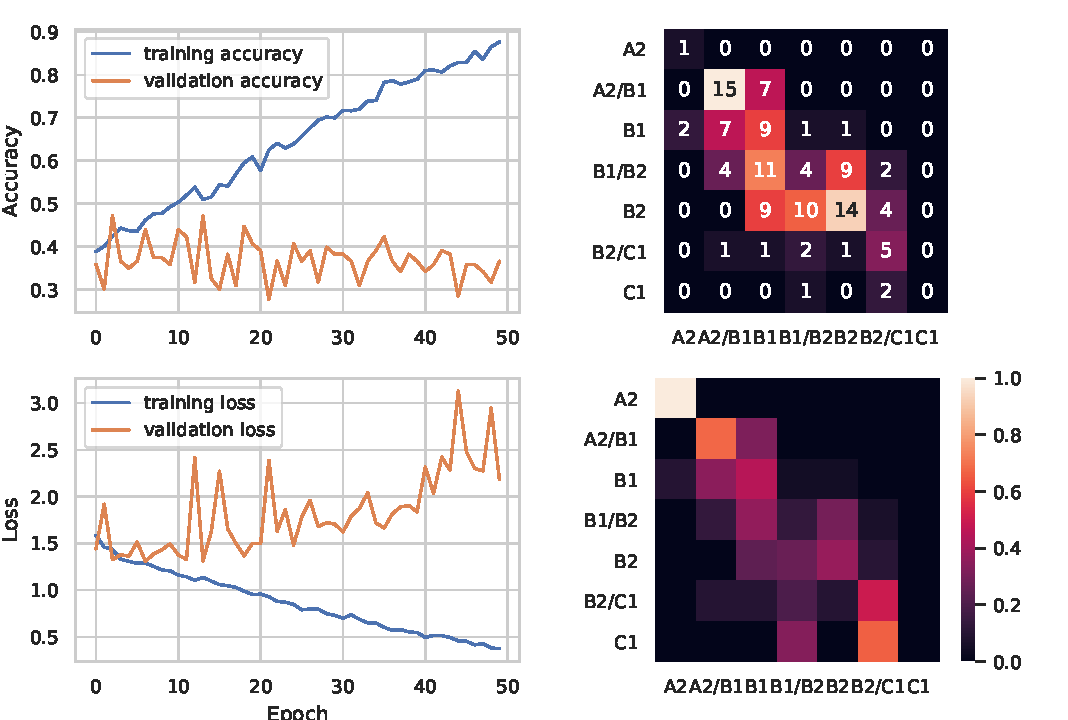
\includegraphics[width=\textwidth]{lstm-training}
  \caption{Training and validation loss and accuracy over 50 epochs of training.
           Also, confusion matrices with counts and normalized by class.}
  \label{fig:lstm-training}
\end{figure}

We see the training and classification of the best RNN model in figure
\ref{fig:lstm-training}, namely the GRU cell with pre-trained, fine-tuned
embeddings and an attention mechanism. It is plain to see that the model
overfits while the validation performance fluctuates. The validation metrics
seem to fluctuate more than they did with the CNN model in fig
\ref{fig:cnn-training}. However, the training accuracy seems to increase
slower, and does not quite reach 100\% in the course of 50 epochs.


\section{Native language identification}

Unlike the proficiency labels in ASK, \ac{L1}s are rather evenly distributed.

We train the same models to classify the documents by native language. The
performance of a \ac{CNN} model improved drastically when including \ac{POS}
tags as input, as evident in table \ref{tab:cnn-nli-results}.

A RNN was able to outperform the CNN only slightly, and here it was not the
attention model that was best, but a bidirectional LSTM.

\begin{table}
  \centering
  \begin{tabular}{lrr}
    \toprule
    Model     & Macro \FI      & Micro \FI \\
    \midrule
    Tokens    &         $0.367$  &         $0.366$  \\ % cnn-nli-2019-02-05_12-54-51
    +POS      & $\mathbf{0.467}$ & $\mathbf{0.463}$ \\ % cnn-nli-2019-01-30_15-32-28
    Mixed POS &         $0.336$  &         $0.333$  \\ % cnn-nli-02-11_16-15-54
    \bottomrule
  \end{tabular}
  \caption{\FI scores of CNN classifiers on NLI}
  \label{tab:cnn-nli-results}
\end{table}

\begin{table}
  \centering
  \begin{tabular}{lrr}
    \toprule
    Model     & Macro \FI      & Micro \FI \\
    \midrule
    Mean/Time &         $0.379$  &         $0.390$  \\ % rnn_nli-25740792
    BiLSTM    & $\mathbf{0.468}$ & $\mathbf{0.480}$ \\ % rnn_nli-25740786
    Attention &         $0.423$  &         $0.407$  \\ % rnn_nli-25740789
    \bottomrule
  \end{tabular}
  \caption{\FI scores of RNN classifiers on NLI}
  \label{tab:rnn-nli-results}
\end{table}

The attention model allows us to visualize the weights the network gives to
each token in a document. In figures
\ref{fig:h0186-nli-attention}--\ref{fig:s0621-nli-attention} we see up to 300
tokens of texts from four different documents in the dev set for which the L1
was correctly predicted by an attention model. Red tokens indicate timesteps
that were given higher weight by the attention model, and blue tokens ones
that were given low weights. Out of vocabulary tokens are replaced by the
special token ``UNK''. The attention values do not seem easily interpretable,
as there are lexical and grammatical errors both in the red and the blue
sections.

Looking for cues as to what features are picked up by the model. \todo{expand analysis}

\begin{figure}
  \centering
  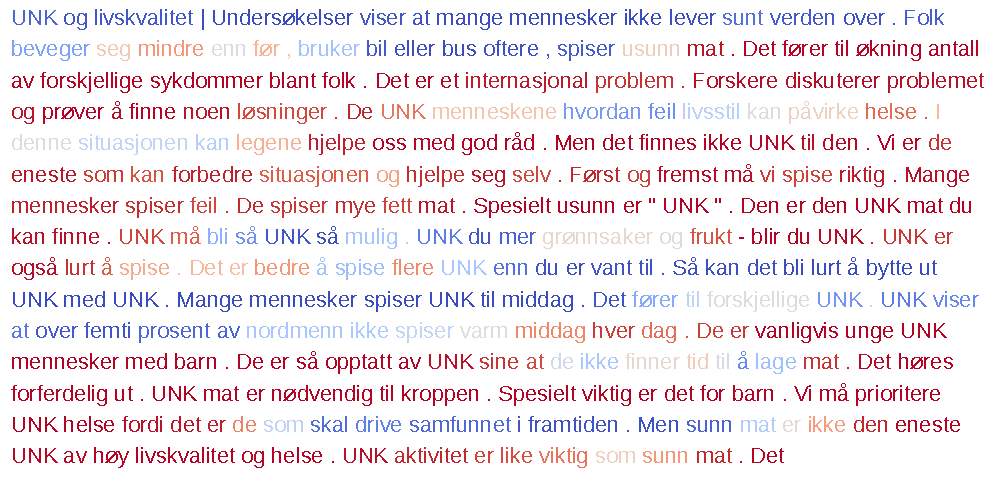
\includegraphics[width=\textwidth]{h0186-nli-attention}
  \caption{Attention values of NLI classifier on excerpt from ASK text h0186.
           L1 is Russian, CEFR score B2}
  \label{fig:h0186-nli-attention}
\end{figure}

\begin{figure}
  \centering
  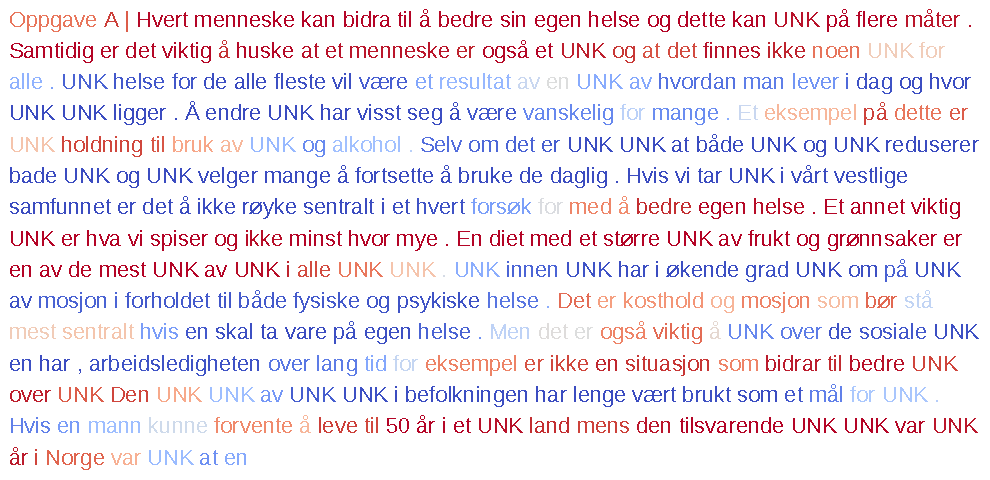
\includegraphics[width=\textwidth]{h0189-nli-attention}
  \caption{Attention values of NLI classifier on excerpt from ASK text h0189.
           L1 is English, CEFR score C1}
  \label{fig:h0189-nli-attention}
\end{figure}

\begin{figure}
  \centering
  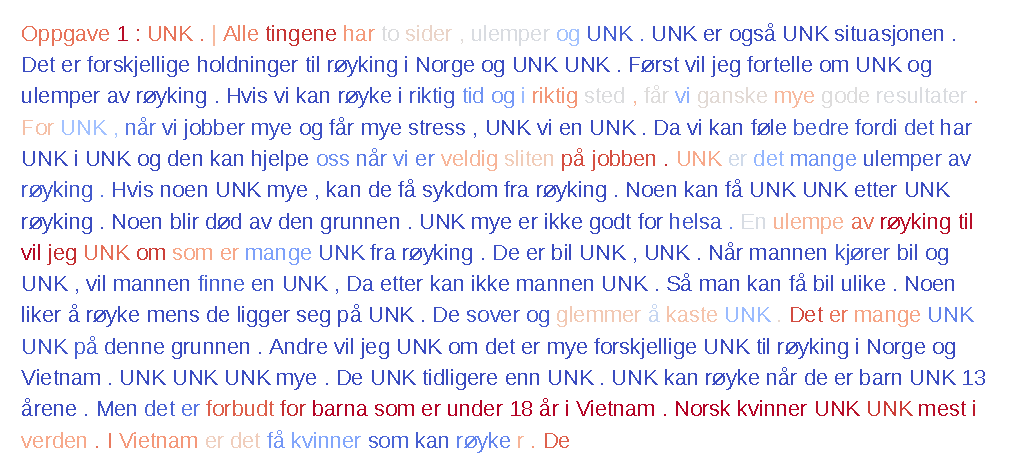
\includegraphics[width=\textwidth]{s0180-nli-attention}
  \caption{Attention values of NLI classifier on excerpt from ASK text s0180.
           L1 is Vietnamese, CEFR score A2/B1}
  \label{fig:s0180-nli-attention}
\end{figure}

\begin{figure}
  \centering
  
\includegraphics[width=\textwidth]{s0621-nli-attention}
  \caption{Attention values of NLI classifier on full ASK text s0621.
           L1 is Somali, CEFR score A2/B1}
  \label{fig:s0621-nli-attention}
\end{figure}
\todo{Visualize UPOS tags}
